\documentclass{article}

\usepackage{graphicx}
\usepackage[margin=1in]{geometry}
\usepackage{amsmath}
\usepackage[T1]{fontenc}
\usepackage[utf8]{inputenc}
\usepackage{authblk}

\begin{document}


\title{Surprisal, Entropy and the N400: \\
Human behavior and language models}

\author[1]{Chris Neufeld}
\author[2]{Benjamin Bengfort}
\affil[1]{Department of Linguistics, University of Maryland}
\affil[2]{Department of Computer Science, University of Maryland}
\affil[ ]{\textit{\{neufeldc,bengfort\}@umd.edu}}

% make the title area
\maketitle

\section*{Abstract}

This paper investigates the extent to which N400 amplitudes are modulated by word predictability and the degree of constraint of the word's environment. In particular, this paper examines whether 'constraint' is best operationalized as the probability of the most likely word in a given context, as is standard in the literature, as the entropy of the probability distribution of words which may appear in that context, or a combination of the two. In addition, we examine whether there are any differences to be found by modeling N400 amplitudes as a function of probabilistic variables derived from cloze data, or from a language model. This paper shows that both entropy and maximum contextual probability interact, modulating the N400 effect. It is further reported that N400 amplitudes are better modeled using data from a cloze procedure than from a language model. These findings are taken to suggest that online linguistic predictions in humans may be subtly modulated by different statistical properties of the incoming signal, above and beyond how probable the most likely following word is given a particular context.


\section{Introduction}


The N400 ERP component has been identified with aspects of lexical prediction and sentential integration in online linguistic processing. The precise cognitive mechanisms underlying this electrophysiological event remain controversial (see \cite{kutas2000electrophysiology} for a review), but it has been well-established that the amplitude of this component is modulated by context. In particular, it has been observed that N400 amplitude stands in a monotonic relationship to the cloze probability of individual words \cite{kutas1984brain}. Words with high cloze probabilities tend to elicit lower N400s than those with low cloze probabilities. More recent work has sought to disambiguate the relationship between the degree of sentence constraint, cloze probability and N400 amplitude. Federmeier and Kutas demonstrate that the degree of contextual constraint interacts with the expectedness of individual words \cite{federmeier1999rose}, a finding replicated in \cite{federmeier2007multiple} Federmeier et al, 2007 (and contrary to earlier reports such as \cite{kutas1984brain} Kutas and Hillyard, 1984).

The degree of contextual constraint in these experiments is typically operationalized in terms of cloze probabilities. For instance, Federmeier et al (2007) \cite{federmeier2007multiple} operationalize sentential constraint in terms of the maximum value in the cloze distribution. They write, “For expected endings [of sentences], cloze probability and constraint cannot be dissociated, since, by definition, only strongly constraining sentences lead to high cloze probability completions.” This does not seem to be strictly true if we take a broader understanding of the meaning of ‘constraint’. It is trivial to construct counter-examples to this assertion: suppose that for both context A and context B, the most probable word in a cloze task is 95\%, but in context A the remaining probability mass is spread among ten words, while in context B, the remaining 5\% is spread among 100 words. Hypothetically, it seems that we would want to say that context A is more constraining than context B, since there are fewer words overall which it supports as a completion.

An alternative operationalization of contextual constraint, independent from the maximum value of the cloze distribution might be the entropy of the cloze distribution. Entropy is an information theoretic quantity which expresses the amount of uncertainty in an information channel in terms of bits.  Entropy is a global property of a particular system which can take on many possible states, rather than a property of any particular state of that system. For example, the probability of getting 1 Head and 1 Tail from flipping two coins is the same as getting Heads from flipping one  coin (state), but the 2-coin system has 2 bits of entropy, while the 1-coin system has 1 bit (system). Entropy seems to be an interesting alternative means of operationalizing contextual constraint in two ways. Firstly, as noted above, it is a global measure of the cloze distribution, rather than simply the maximum value. Secondly, it seems conceptually closer to the notion of constraint since it is a precise mathematical formalization of the average amount of information gained when receiving a message (here, word), from a particular channel (sentence context). A very highly constraining context can be conceptualized as an information channel with very low entropy: we receive almost no new information upon hearing ‘friend’ after hearing ‘A dog is a man’s best...’, while we receive a lot more information upon hearing ‘friend’ after hearing ‘I went to meet my...’

Further, we have some intuition from our readings in the computational space that entropy is primary evaluation of computational language models- namely the perplexity of a model. If the N400 is modulated based on the entropy of the cloze probability then it would seem that the evaluation of the language models on perplexity is indeed on the right track, and we should compare the surprisal of the model to the amplitude of the N400 to find algorithms that are truly in line with the human experience of semantic understanding as in \cite{frank2013word} (Frank, 2013). If the entropy does affect humans perception of the predicted next word, perhaps this can help us build better language models. Therefore in addition to our study of N400 modulation in relation to cloze probabilities, we also will compare the modulation of N400 to probability distributions in other language models, using the two canonical models we have seen so far- a back-off model and a connectionist model similar to the work done in \cite{frank2009surprisal,demberg2009computational}. We should note that other models do exist, as in the top-down incremental parser in \cite{roark2009deriving} but we are attempting to isolate semantic contextual effects from the syntactic ones. 

In order to explore these ideas, N400 amplitudes are modeled as a function of three quantities: the bigram probability of a word, given a preceding context, the probability of the most likely item in a given context, and the entropy of the probability distribution of all possible words of a given context. If linguistic predictions are modulated by the entropy of a given context, we would predict that entropy would be a significant component of the model. If, however, constraints on linguistic prediction are explained only by the probability of the most likely subsequent item, we expect that entropy not be a significant predictor of N400 amplitude.

\section{Methods}

EEG data and materials were taken from \cite{lau2014}, and the reader is referred to that paper for more detailed descriptions of the materials used, and the parameters of the EEG data collection. In brief, materials were 240 adjective-noun sequences with a range of bigram probabilities and a range of contextual constraint. For that paper, constraint was operationalized as the maximum probability of a noun, given an adjective frame. Bigram probabilities were estimated from the Corpus of Contemporary American English \cite{davies2008} as well as the Microsoft Web N-Gram Corpus \cite{wang2010overview}. Corpus probabilities were calculated using a Kneser-Ney smoothed \cite{kneser1995improved} bigram model. EEG subjects were visually presented with adjective-noun pairs, and were intermittently given a memory test to ensure their continued attention to the stimuli. 

\subsection{Cloze data}

Cloze data for the experimental materials were gathered using Amazon Mechanical Turk. Participants were given prompts of an adjective, and instructed to supply the word which best followed the prime. Data were collected from 37 participants. For each adjective-noun pair in the experimental materials, the following quantities were computed from the cloze data:

\begin{itemize}
\item $P$: The bigram probability of the target nouns, given the preceding adjective: $p(noun|adjective)$
\item $maxP$ The highest bigram probability for a given adjectival context: $max(P)$
\item $H$: The entropy of the distribution of bigram probabilities for a given adjectival context: $-\sum{}Plog_2P$
\end{itemize}

\subsection{Language modeling}

Several corpora in different domains were evaluated for their suitability in building a language model that would closely approximate the model generated by the cloze task. The cloze task contained 558 adjectival prompts and returned 2178 noun responses in 5328 adjective-noun bigrams. In order to evaluate the correlation of the independent variables in the corpus data to the cloze data in particular we wanted to ensure that the corpus had a significant coverage of these adjectives, nouns, and adjective-noun pairs. Our initial evaluations of smaller million word corpora revealed that this task would not be particularly easy, as different types of discourse rely on different language structures. Table \ref{tab:corpora_comparison} shows several corpora and the percent of intersection with the cloze task.

\begin{table}[t!]
    \centering
    \caption{Intersection of Corpora with Cloze Data}
    \label{tab:corpora_comparison}
    \begin{tabular}{l | c c c c c}
        \hline
        Corpus & Vocabulary & Adjectives & Nouns & Exact Bigrams & Bigrams \\
        \hline
        Reuters & 64.95\% & 47.49\% & 69.47\%& 2.08\% & 67.38\% \\
		Web Text & 66.67\% & 38.17\% & 74.01\% & 1.33\% & 24.71\% \\
		Literature & 81.03\% & 68.64\% & 84.25\% & 3.19\% & 125.47\% \\
		Brown & 89.19\% & 81.00\% & 91.32\% & 5.18\% & 95.25\% \\
		Treebank & 48.10\% & 26.34\% & 53.76\% & 0.51\% & 9.21\% \\
		BWAC & 92.75\% & 89.43\% & 93.57\% & 10.34\% & 302.68\% \\
		COCA & 81.39\% & 70.07\% & 84.34\% & 16.35\% & 100.84\% \\
        \hline
    \end{tabular}
\end{table}

In the end we decided that the Corpus of Contemporary American English \cite{davies2008} would be the ideal selection for the manual construction of both the connectionist and sequential models for further research, and would be the selection to continue this work. For the purposes of our initial investigation, whose results we report in this paper, we used the far more comprehensive \textit{Microsoft Web N-Gram Corpus} \cite{wang2010overview}, a billion word corpus that has complete coverage of the vocabulary and ngrams in the cloze data. The same independent variables $P$, $maxP$ and $H$ were evaluated for the corpus data using a Kneser-Ney smoothed bigram model. Dot plotted distributions of interest for both the cloze and corpus data set are plotted in Figure \ref{fig:probability_distributions} - showing the relationship between entropy and constraint as operationalized in N400 tasks. The word "wrought" is highly constraining and has a very low entropy. The adjective "disposable" is considered to have a low constraint, and has a comparatively high entropy. But how constraint is operationalized relative to entropy is suggested by the "buttered" distribution - an adjective that is typically thought of as highly constraining, but also has a fairly high entropy.

\begin{figure}
	\centering
	\begin{minipage}{0.33\textwidth}
		\centering
    		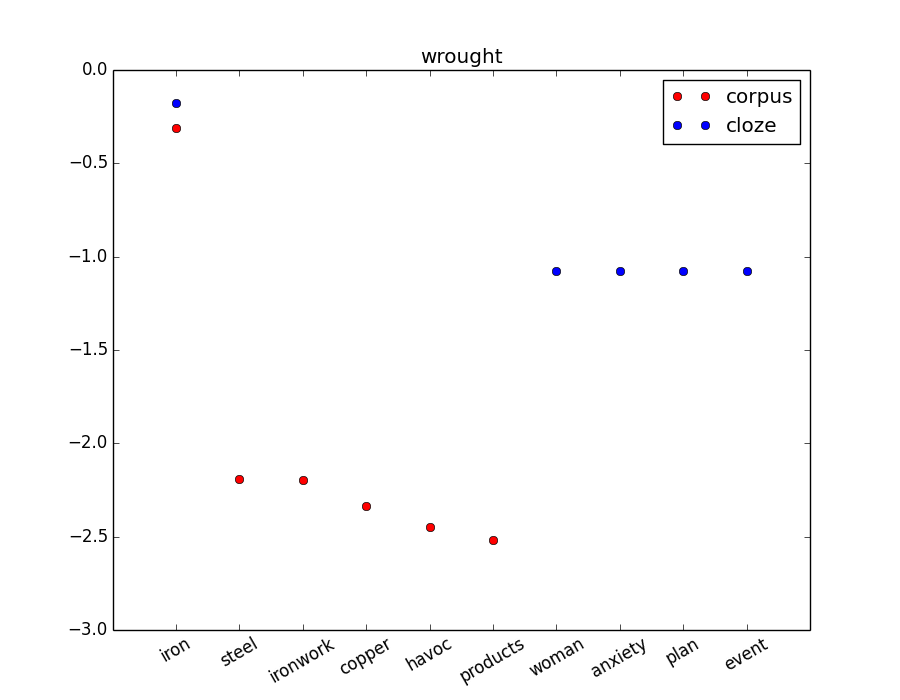
\includegraphics[width=\textwidth]{figures/wrought_dist}
	\end{minipage}%
	\begin{minipage}{0.33\textwidth}
		\centering
    		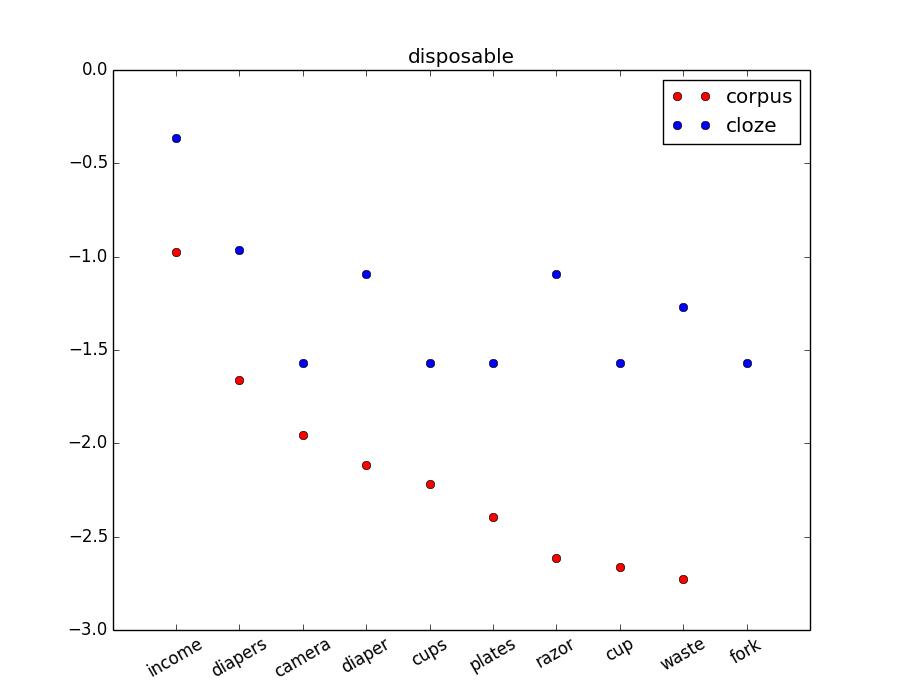
\includegraphics[width=\textwidth]{figures/disposable_dist}
	\end{minipage}
    \begin{minipage}{0.33\textwidth}
		\centering
    		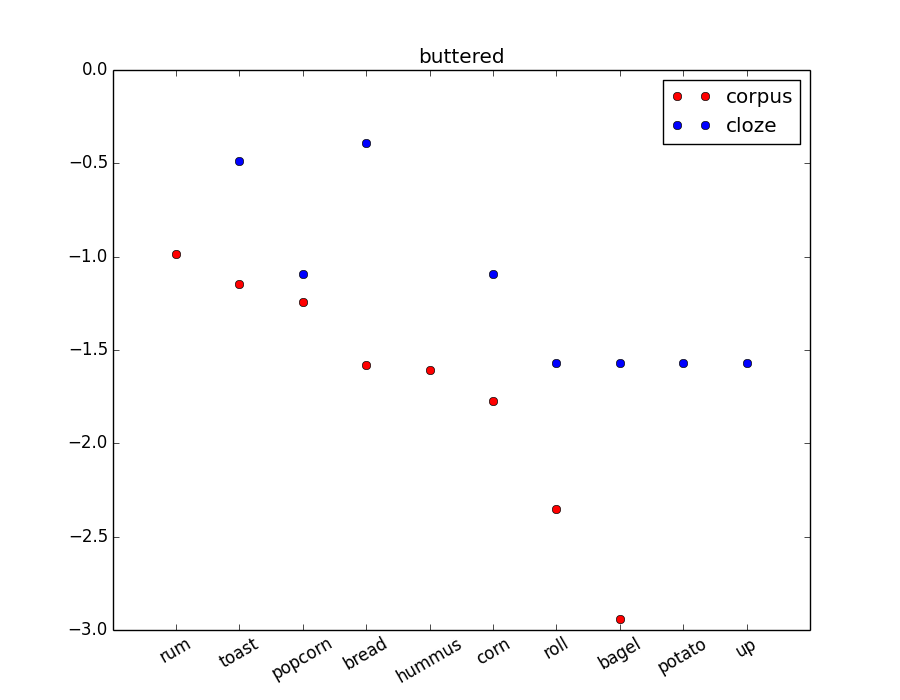
\includegraphics[width=\textwidth]{figures/buttered_dist}
	\end{minipage}
	\caption{Dot plots of the probabilities from the cloze and corpus data representing the relationship between entropy and constraint. For example "wrought" has a highly constraining, low entropy probability distribution. "Disposable" is considered low constraint and has a high entropy. Of interest is the high entropy but highly constraining "buttered" distribution.}
    \label{fig:probability_distributions}
\end{figure}


\subsection{EEG data analysis}

EEG analysis focused exclusively on the electrophysiological response to the noun. The vertex CZ electrode was chosen for analysis. EEG data were epoched 100 ms pre-stimulus, and 1000 ms post-stimulus. Trials with myogenic and ocular artifacts were automatically detected and excluded from analysis. The remaining EEG timeseries were filtered with an 11-point Butterworth band-pass filter with a 1-30 Hz pass-band. Each voltage timeseries was baselined by subtracting the mean voltage of the pre-stimulus interval. For each subject, EEG voltage timeseries were averaged across all conditions at each timestep. The resulting event-related potential was inspected visually, and the N400 was identified as a large local minima in the ERP occurring around 400 ms, and the latency of the N400 was recorded for each subject for subsequent analysis. The mean N400 latency was 377.8 ms, and standard deviation was 36.6 ms. These latencies are recorded in table \ref{tab:latencies} in the Appendix. An example ERP waveform from one subject is shown in figure \ref{fig:egERP}, and the grand mean ERP, averaged across all stimuli and subjects, is shown in figure \ref{fig:grandERP}.

After excluding artifacts, only those stimuli which had 20 or more viable EEG timeseries were included for analysis. N400 amplitudes for each stimulus were estimated as follows. Each subject's mean N400 latency was retrieved. For each stimulus which that subject was presented, voltage values were extracted from a 200 ms window centered around the subjects' mean N400 latency, and averaged. This window size was chosen by examining how the correlation between bigram probability, $P$, and N400 amplitude varied as a function of window size. In order not to privilege the corpus or cloze data, the value of $P$ was averaged across both data sets within each item. The window size which maximized the correlation between N400 amplitude and $P$ was selected. Although this window size is relatively large in comparison to standard values in the ERP literature, it may be that within-subject phase-variability in the N400 response in single trials necessitated a relatively large window to capture the event-related negativity. These voltage values were then averaged across subjects for each item. Since each stimulus was only presented to each subject at most once, centering the time window around subject-specific N400 latency was necessary to compute a meaningful estimate of the N400 amplitude for that specific stimuli. Small cross-subject variability in the phase of the N400 response can easily wipe out the effects since each subject contributes only one trial to the estimation of N400 amplitude for any particular stimuli.


\begin{figure}
	\centering
		\includegraphics{figures/example_N400}
	\caption{Example event-related potential for one subject, averaged across all stimuli. The latency of the N400 is indicated by a vertical dashed line. Negative is plotted up.
    \label{fig:egERP}}
\end{figure}

\begin{figure}
	\centering
		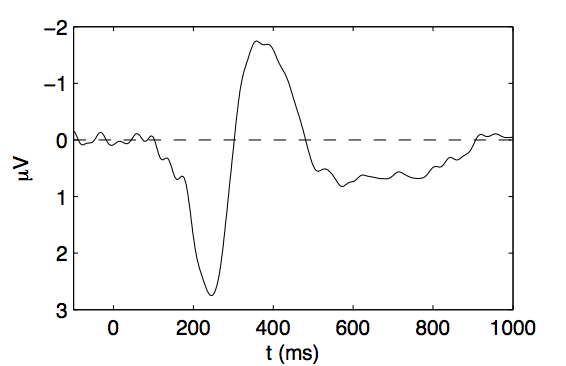
\includegraphics{figures/grand_N400}
	\caption{Grand-average event-related potential, averaged across all subjects and stimuli. 
    \label{fig:grandERP}}
\end{figure}


\section{Results}

Figure \ref{fig_dependent} graphically depicts the relationship between N400 amplitudes and the dependent variables selected here for examination. As expected, N400 amplitude is correlated with cloze bigram probability, with less probable words eliciting a greater negativity. N400 amplitudes appear positively correlated with $maxP$, and negatively correlated with $H$.

\begin{figure}
\begin{centering}
\includegraphics{figures/dependent}
\caption{Relationship between N400 amplitude and dependent variables $P$, $maxP$ and $H$. The left column shows the relationship for dependent variables derived from cloze data, and the right column shows data derived from corpus data. A line of best fit is printed for each plot. The relationship between N400 and $P$ from the cloze data is shown in a log-scale for visual clarity, but the analysis is conducted on a linear scale (see body text for more details). \label{fig_dependent}}
\end{centering}
\end{figure}

Figure \ref{fig_independent} depicts the relationship between the various dependent variables under study, for both the cloze and corpus data.

\begin{figure}
	\centering
		\includegraphics{figures/independent_variables}
	\caption{\textbf{A}: relationship between dependent variables within data source. The left column shows the relationship for the cloze data, and the right column shows the corpus data. Strong linear relationships can be observed for all variables from the cloze data. For the corpus data, the relationship between $H$ and $maxP$ is clearly linear as well, though not so for the other combinations of variables. \textbf{B}: relationship between cloze and corpus data, within each dependent variable.  Corpus and cloze data appear to be relatively uncorrelated. As in \ref{fig_dependent}, axes with $P$ are shown in log-scale for the corpus data. 
    \label{fig_independent}}
\end{figure}

For both the cloze data and corpus data, we faced a choice whether to express the conditional probabilities $P$ and the maximum probabilities $maxP$ in a linear or log scale. In language modeling, probabilities are typically expressed in a logarithmic scale -- however, we had no \emph{a priori} reason to assume that N400 amplitudes would be best modeled as an effect of variables in a linear or log scale. To test this hypothesis, for both corpus and cloze data, separate general linear models (GLMs) were constructed regressing N400 amplitudes against $P$, $maxP$ and $H$, with $P$ and $maxP$ expressed in both linear and logarithmic scales. For both the cloze and corpus data, the linear model constructed from predictors expressed in a linear scale was a better fit that the model constructed with predictors in a log scale. Each linear model was tested against a null model using an F-test. The adjusted $R^2$ (a measure of goodness-of-fit) and the results of the F-tests are reported in table \ref{tab_gof}. For both Cloze and Corpus linear models, the fit to the data is better with regressors in a linear scale (higher $R^2$, lower $p$-values). Since the models constructed with linear predictors are better overall, all subsequent analysis uses this scale.


\begin{table}
	\centering
	\caption{Goodness-of-fit for GLMs \label{tab_gof}}
	\begin{tabular}{ll|cccc}
		&						&	Adjusted $R^2$	&	F	&	d.f.	&	$p$\\
        \hline
        \hline
Cloze	&	Linear regressors	&	0.13			&	5.31 &	7,192 & $<0.00001$\\
		&	Log regressors		&	0.08			&	3.366 & 7,192 & $<0.005$\\
\hline
Corpus	&	Linear regressors	&	0.011			&	1.327 & 7,192 & 0.24\\
		&	Log regressors		&	-0.003			&	0.9172	& 7,192 & 0.49
	\end{tabular}
\end{table}


Because the corpus model is not significantly better than a null model, further analysis is confined to examining the cloze model. We will return to this point in the discussion, but since the best GLM for the corpus data is effectively random, there is nothing to be gained by analyzing the model further. The parameters of the (more successful) cloze model are summarized in table \ref{tab_glm_summary}. According to the t-tests summarized in this table, only $P$ and all three interaction terms are significant components of the model. This conforms to our basic intuition that, (1), N400 amplitudes vary primarily as a function of probability, and (2) that this effect is modulated by the degree of constraint, as shown by the significance of the interaction terms. However, these tests do not address whether it is $maxP$, $H$ or both which is the more appropriate measure of constraint since, as discussed above, these two variables are quite correlated. 



\begin{table}
\centering
	\caption{Summary of GLM constructed for cloze data \label{tab_glm_summary}}
	\begin{tabular}{l|cccc}
							&	Coefficient	&	Standard Error	&	$t$-value 	&	$p$\\
                            \hline
(Intercept)                 &	-2.8		&	2.36			&	1.18		&	0.24\\
$P$							&	15.14		&	7.17			&	2.11		&	$\mathbf{<0.05}$\\
$maxP$						&	0.77		&	2.65			&	0.29		&	0.77\\
$H$							&	0.37		&	0.50			&	0.76		&	0.45\\
$P\times{}maxP$				&	-15.03		&	7.16			&	2.10		&	$\mathbf{<0.05}$\\
$P\times{}H$				&	-3.7		&	1.67			&	2.22		&	$\mathbf{<0.05}$\\
$maxP\times{}H$				&	-0.53		&	0.73			&	-0.72		&	0.47\\
$P\times{}H\times{}maxP$	&	3.80		&	1.49			&	2.55		&	$\mathbf{<0.05}$\\
	\end{tabular}
\end{table}

We performed a statistical analyses on this GLM to determine the extent to which $H$ and/or $maxP$ modulate N400 amplitude, and to address our central question of how best to operationalize the constraint of a linguistic context. In this analysis, the full GLM for the cloze data is built sequentially, and with each added term, the Chi-square statistic is evaluated to assess whether the regressor significantly decreases the deviance of the model. This procedure has the effect of decorrelating the highly correlated dependent variables in the cloze data set. If a term is added to the model which is highly correlated with the already-incorporated terms, but there is nevertheless a significant decrease in model deviance, then we may conclude that, despite the strong relationship between terms, there exists some component of the term orthogonal to the covariation which is a good predictor of the (in this case, N400) data.
The results of this procedure are shown in \ref{tab_seq}. $P$ is, unsurprisingly, a highly significant predictor of N400. However, with the addition of each subsequent term, there is no significant decrease in model deviance until the addition of the final cubic term, $P\times{}maxP\times{}H$. Since different $p$-values for particular terms are obtained depending on the order in which terms are added, we also performed the same sequence of tests with the order of $maxP$ and $H$ reversed. We obtained the same result: after the addition of the first term, only the 3-way interaction term significantly decreased model deviance. This result may be interpreted that \emph{both} $maxP$ and $H$ modulate the relationship between N400 amplitude and $P$, and that they do so in an interactive fashion.

This interaction is represented graphically in \ref{fig_interaction}. This figure shows portions of the GLM. Since it is a function of three independent variables, here we depict surfaces resulting from evaluating the GLM at a single low-entropy value and a single high-entropy value.

In high-entropy contexts (relatively low `constraint), the classic effect holds: If the environment is highly constraining (high $maxP$), then  unpredicted words elicit a larger N400. However, in low-entropy contexts, something quite different is seen. If the environment is highly constraining (high $maxP$), then N400 magnitude \emph{decreases} with respect to the word's probability. If the environment is less constraining, then (low $maxP$), then N400 amplitude is essentially flat with respect to target probability.


\begin{figure}
	\centering
		\includegraphics{figures/interaction}
	\caption{Graphical representation of the GLM modeling N400 amplitude as a function of $P$, $maxP$ and $H$. The left panel shows the surface resulting from evaluating the model at a low $H$ value, and the right panel shows the surface resulting from evaluating the model at a high $H$ value. In high entropy contexts, the classic effect of constraint is observed: N400 amplitudes vary as a function of word probability in high-$maxP$ environments, and the effect is relatively flat in low-$maxP$ environments. In low entropy-environments, the opposite effect is seen: N400 amplitude varies inversely as a function of word probability in high-$maxP$ environments, though is still relatively flat in low-$maxP$ environments. 
    \label{fig_interaction}}
\end{figure}




\begin{table}
	\centering
	\begin{tabular}{l|ccccc}
							&	d.f.	&	Deviance	&	Residual d.f.	&	 Residual Deviance	&	$p$\\
                        \hline             
NULL					&				&				&	199				&	435.75\\
$P$						&	1			&	46.33		&	198				&	389.41				&	$\mathbf{<10^{-7}}$\\
$maxP$					&	1			&	5.31		&	197				&	384.1				&	0.9\\
$H$						&	1			&	1.59		&	196				&	382.51				&	0.36\\
$P\times{}maxP$			&	1			&	2.08		&	195				&	380.43				&	0.30\\
$P\times{}H$			&	1			&	2.54		&	194				&	377.9				&	0.25\\
$maxP\times{}H$			&	1			&	0.51		&	193				&	377.39				&	0.60\\
$P\times{}maxP\times{}H$&	1			&	12.33		&	192				&	365.05				&	$\mathbf{<0.05}$
	\end{tabular}
    \caption{Summary of sequential GLM construction. Each line shows the effect of adding that term to the model. After the addition of the conditional probability of the word, $P$, as a predictor of N400, no term significantly decreases the residual deviance according to a Chi-square test except for the final cubic term $P\times{}maxP\times{}H$ 
    \label{tab_seq}}
\end{table}


\section{Discussion \& Conclusion}

The findings outlined above are largely in conformity with the findings of the ERP literature: the classic N400 effect is modulated by the degree of constraint of the environment. Highly-constraining environments elicit a larger N400 in response to an non-predicted word, where constraint is operationalized as the probability of the most likely subsequent word. Further, the results from this investigation suggest that the basic interaction is modulated still further by the entropy of the distribution of \emph{all} possible subsequent words; and that entropy, maximum contextual probability, and contextual probability all interact in a relatively complex fashion. If the N400 is understood as an index on linguistic predictions, these results suggest that human predictive processing may be guided not only by coarse statistical quantities (how likely is the next most likely thing), but also by global heuristics computed over the space of possible continuations of the linguistic utterance, such as entropy. 

This result may be slightly overshadowed by the fact that we did not get a strong correlation between the N400 response and the likelihoods as computed by the language models constructed from the Microsoft Web N-Gram corpus, a fact which contradicts the work of of Smith \& Levy in \cite{smith2011cloze} who suggest that corpus data more accurately reflects the N400 response then the typical cloze task. Furthermore using the COCA corpus, current work by Lau, Fogel, and Delgado has found a correlation between N400 response and the same adjective-noun data that we used in our data set. A technical inspection of our computations may be necessary, but it is worth investigating what effect a billion word web-domain corpus may have on correlative values. Perhaps there is an upper limit to the amount of information required to build a language model that actually reflects human experience of linguistic processing. The Web corpus contained extremely large distributions of noun completions, although we did not filter on part of speech (e.g. this is an adjective, produce a noun) - for example the bigram "wrought havoc" (a verb phrase) appeared in our corpus. Further investigation and a validation by building language models from the COCA data set is required.

This paper examined very simple linguistic contexts, with the predictability and constraint of words being controlled only by a single adjective. As a first step, this seems like a natural place to start, as the electrophysiological record and language modeling are unencumbered by syntactic structure \cite{kim2005}, discourse context \cite{otten2007}, working memory \cite{vanpetten1997}, temporal dynamics \cite{chowinprep}, or other higher-order processes linguistic processes known to exert effects on N400 amplitudes. However it would be interesting to extend this style of analysis to more complex linguistic materials, in particular to examine whether the complex interaction between contextual entropy and maximum probability, and word-probability extends to more linguistically sophisticated environments, or whether the effect is confined to more limited contexts where the predictive computations involved are presumably less taxing, both for language models, as well a humans.


\pagebreak

\bibliographystyle{plain}
\bibliography{paper}

\section*{Appendix}

\begin{table}
\caption{\label{tab:latencies}N400 latencies by subject}
\begin{tabular}{c|c}
Subject & Latency\\
\hline1&380\\
2&401\\
3&340\\
4&375\\
5&377\\
6&423\\
7&372\\
8&363\\
9&359\\
10&391\\
11&373\\
12&460\\
13&395\\
14&377\\
15&312\\
16&329\\
17&439\\
18&389\\
19&403\\
20&391\\
21&345\\
22&359\\
23&323\\
24&321\\
25&361\\
26&387\\
27&415\\
28&360\\
29&381\\
30&435\\
31&363\\
32&439\\
33&409\\
34&365\\
35&321\\
36&415\\
37&391\\
38&319
\end{tabular}
\end{table}

\end{document}

